\documentclass[a4paper, 11pt, oneside]{article}

\usepackage[utf8]{inputenc}
\usepackage[T1]{fontenc}
\usepackage[french]{babel}
\usepackage{array}
\usepackage{shortvrb}
\usepackage{listings}
\usepackage[fleqn]{amsmath}
\usepackage{amsfonts}
\usepackage{fullpage}
\usepackage{enumerate}
\usepackage{graphicx}             % import, scale, and rotate graphics
\usepackage{subfigure}            % group figures
\usepackage{alltt}
\usepackage{url}
\usepackage{indentfirst}
\usepackage{eurosym}
\usepackage{listings}
\usepackage{color}
\usepackage[table,xcdraw,dvipsnames]{xcolor}


% Change le nom par défaut des listing
\renewcommand{\lstlistingname}{Extrait de Code}

% Change la police des titres pour convenir à votre seul lecteur
\usepackage{sectsty}
\allsectionsfont{\sffamily\mdseries\upshape}
% Idem pour la table des matière.
\usepackage[nottoc,notlof,notlot]{tocbibind}
\usepackage[titles,subfigure]{tocloft}
\renewcommand{\cftsecfont}{\rmfamily\mdseries\upshape}
\renewcommand{\cftsecpagefont}{\rmfamily\mdseries\upshape}

\definecolor{mygray}{rgb}{0.5,0.5,0.5}
\newcommand{\coms}[1]{\textcolor{MidnightBlue}{#1}}

\lstset{
    language=C, % Utilisation du langage C
    commentstyle={\color{MidnightBlue}}, % Couleur des commentaires
    frame=single, % Entoure le code d'un joli cadre
    rulecolor=\color{black}, % Couleur de la ligne qui forme le cadre
    stringstyle=\color{RawSienna}, % Couleur des chaines de caractères
    numbers=left, % Ajoute une numérotation des lignes à gauche
    numbersep=5pt, % Distance entre les numérots de lignes et le code
    numberstyle=\tiny\color{mygray}, % Couleur des numéros de lignes
    basicstyle=\tt\footnotesize,
    tabsize=3, % Largeur des tabulations par défaut
    keywordstyle=\tt\bf\footnotesize\color{Sepia}, % Style des mots-clés
    extendedchars=true,
    captionpos=b, % sets the caption-position to bottom
    texcl=true, % Commentaires sur une ligne interprétés en Latex
    showstringspaces=false, % Ne montre pas les espace dans les chaines de caractères
    escapeinside={(>}{<)}, % Permet de mettre du latex entre des <( et )>.
    inputencoding=utf8,
    literate=
  {á}{{\'a}}1 {é}{{\'e}}1 {í}{{\'i}}1 {ó}{{\'o}}1 {ú}{{\'u}}1
  {Á}{{\'A}}1 {É}{{\'E}}1 {Í}{{\'I}}1 {Ó}{{\'O}}1 {Ú}{{\'U}}1
  {à}{{\`a}}1 {è}{{\`e}}1 {ì}{{\`i}}1 {ò}{{\`o}}1 {ù}{{\`u}}1
  {À}{{\`A}}1 {È}{{\`E}}1 {Ì}{{\`I}}1 {Ò}{{\`O}}1 {Ù}{{\`U}}1
  {ä}{{\"a}}1 {ë}{{\"e}}1 {ï}{{\"i}}1 {ö}{{\"o}}1 {ü}{{\"u}}1
  {Ä}{{\"A}}1 {Ë}{{\"E}}1 {Ï}{{\"I}}1 {Ö}{{\"O}}1 {Ü}{{\"U}}1
  {â}{{\^a}}1 {ê}{{\^e}}1 {î}{{\^i}}1 {ô}{{\^o}}1 {û}{{\^u}}1
  {Â}{{\^A}}1 {Ê}{{\^E}}1 {Î}{{\^I}}1 {Ô}{{\^O}}1 {Û}{{\^U}}1
  {œ}{{\oe}}1 {Œ}{{\OE}}1 {æ}{{\ae}}1 {Æ}{{\AE}}1 {ß}{{\ss}}1
  {ű}{{\H{u}}}1 {Ű}{{\H{U}}}1 {ő}{{\H{o}}}1 {Ő}{{\H{O}}}1
  {ç}{{\c c}}1 {Ç}{{\c C}}1 {ø}{{\o}}1 {å}{{\r a}}1 {Å}{{\r A}}1
  {€}{{\euro}}1 {£}{{\pounds}}1 {«}{{\guillemotleft}}1
  {»}{{\guillemotright}}1 {ñ}{{\~n}}1 {Ñ}{{\~N}}1 {¿}{{?`}}1
}
\newcommand{\tablemat}{~}

%%%%%%%%%%%%%%%%% TITRE %%%%%%%%%%%%%%%%
% Complétez et décommentez les définitions de macros suivantes :
\newcommand{\intitule}{Polylignes}
\newcommand{\GrNbr}{06}
\newcommand{\PrenomUN}{Maxime}
\newcommand{\NomUN}{Deravet}
\newcommand{\PrenomDEUX}{Luca}
\newcommand{\NomDEUX}{Matagne}
% Décommentez ceci si vous voulez une table des matières :
\renewcommand{\tablemat}{\tableofcontents}

%%%%%%%% ZONE PROTÉGÉE : MODIFIEZ UNE DES DIX PROCHAINES %%%%%%%%
%%%%%%%%            LIGNES POUR PERDRE 2 PTS.            %%%%%%%%
\title{INFO0947: \intitule}
\author{Groupe \GrNbr : \PrenomUN~\textsc{\NomUN}, \PrenomDEUX~\textsc{\NomDEUX}}
\date{}
\begin{document}

\maketitle
\newpage
\tablemat
\newpage
%%%%%%%%%%%%%%%%%%%% FIN DE LA ZONE PROTÉGÉE %%%%%%%%%%%%%%%%%%%%

%%%%%%%%%%%%%%%% RAPPORT %%%%%%%%%%%%%%%
% Écrivez votre rapport ci-dessous.
\section{Remarque sur la compréhension du problème}
Nous nous sommes retrouvez face à une divergence de compréhension sur ce que voulais dire fermer/ouvrir une polyligne. Après une  longue discussion à ce sujet, nous avons décidé que pour nous, fermer une polyligne ne consistait pas juste à relier la cellule du dernier point à la cellule du premier point mais bien à AJOUTER un point en fin de liste ayant LES MEMES coordonnées que le premier point. Cela nous permet d'ajouter un nouveau point à une polyligne déjà fermée par exemple. Il est important de comprendre notre vision de la chose pour comprendre comment fonctionne nos implémentations.


\section{TAD: Point2D}

\subsection{Signature}

\noindent TYPE: Point2D

\noindent UTILISE: Réels 

\noindent OPERATIONS: 
\begin{itemize}
    \item Create: Réels $\times$ Réels $\xrightarrow{}$ Point2D {\color{green} C}\footnote{Les lettres vertes permettront, durant tout ce rapport, de mettre en évidence les observateurs et les opérations internes.}
    \item GetX: $Point2D \xrightarrow{}$ Réels {\color{green} O}
    \item GetY: $Point2d \xrightarrow{}$ Réels {\color{green} O}
    \item EuclDist: $Point2D \times Point2d \xrightarrow{}$ Réels {\color{green} O}
    \item Translate: $Point2D \times Point2d \xrightarrow{} Point2D$ {\color{green} T}
    \item Rotate: $Point2D \times Point2d  \times $ Réels $\xrightarrow{} Point2D $ {\color{green} T}
\end{itemize}



\subsection{Sémantique}
\noindent PRECONDITIONS:

\noindent AXIOMES: 
$\forall X,Y \in Reels$
\begin{itemize}
    \item GetX(Create(a,b)) = a
    \item GetY(Create(a,b)) = b
    \item EuclDist(X,Y) = $\sqrt{{(GetX(X)-GetX(Y))}^{2}+{(GetY(X)-GetY(Y))}^{2}}$
    \item GetX(Translate(U,V)) = GetX(U) + GetX(V)
    \item GetY(Translate(U,V)) = GetY(U) + GetY(V)
    \item GetX(Rotate(U,V,f)) = $cos(f) \times (GetX(U)-GetX(V)) - sin(f) \times (GetY(U)-GetY(V)) + GetX(V) $ 
    \item GetY(Rotate(U,V,f)) = $sin(f) \times (GetX(U)-GetX(V)) + cos(f) \times (GetY(U)-GetY(V)) + GetY(V) $ 
    
    
    
\end{itemize}

\subsection{Structure}
Un point est créé sur base du couple de ses coordonnées (x,y). 

\begin{lstlisting}
struct Point2D{
	float x;
	float y;
};
\end{lstlisting}

\subsection{Fonctions et procédures}

\begin{lstlisting}[escapeinside={(*}{*)}]

/* 
 * @pre: /
 * @post: (get_x(create_Point2D) = x 
 *(* \color{blue}{$\land$} *)
 * get_y(create_Point2D) = y) 
 */
Point2D* CreatePoint2D(float x, float y);
/* 
 * @pre: A != NULL
 * @post: (*$\color{blue}{A=A_0  \land }  get_x = A->x$ *)
 */
float get_x(Point2D* A);
/* 
 * @pre: A != NULL
 * @post: (*$\color{blue}{A=A_0  \land }  get_y = A->y$ *)
 */
float get_y(Point2D* A);
/* 
 * @pre: A != NULL (*\color{blue}{$\land $} *) B != NULL
 * @post: (*$ \color{blue}{A=A_0 \land B=B_0 \land  EuclDist = \sqrt{(X_a-X_b)+(Y_a-Y_b)} } $*)
 */
unsigned float EuclDist(Point2D* A, Point2D* B);
/* 
 * @pre: (*\color{blue}{A != NULL $\land$ B != NULL}*)
 * @post: (*\color{blue}{$A=Translate_{(A, B)} \land B=B_0$}*)
 */
void TranslatePoint2D(Point2D* A, Point2D* B);
/* 
 * @pre: (*\color{blue}{A != NULL $\land$ B != NULL}*)
 * @post: (*\color{blue}{$A=Rotate_{(A, B), x} \land B=B_0 $}*)
 */
void RotatePoint2D(Point2D* A, Point2D* B, float x);
\end{lstlisting}


\section{TAD: Polyligne}

\subsection{Signature}

\noindent TYPE: Polyligne

\noindent UTILISE: Point2D, Réels, Naturels, Boolean


\noindent OPERATIONS: 
\begin{itemize}
    \item Create: $Point2D \times Point2D \times Boolean \xrightarrow{} Polyligne$ 
    \item Close: $Polyligne \xrightarrow{} Polyligne$ {\color{green} T}
    \item Open: $Polyligne \xrightarrow{} Polyligne$ {\color{green} T}
    \item IsOpen: $Polyligne \xrightarrow{} Boolean$ {\color{green} O}
    \item NbrPoint: $Polyligne \xrightarrow{} Naturels$ {\color{green} O}
    \item GetPoint: $Polyligne \times Naturels \xrightarrow{} Point2D$ {\color{green} O}
    \item Length: $Polyligne \times Reels$ {\color{green} O}
    \item AddPoint: $Polyligne \times Point2D \xrightarrow{} Polyligne${\color{green} T}
    \item SuppPoint: $Polyligne \xrightarrow{} Polyligne$ {\color{green} T}
    \item PolyTranslate: $Polyligne \times Point2D \xrightarrow{} Polyligne$ {\color{green} T}
    \item PolyRotate: $Polyligne \times Reels \times Point2D \xrightarrow{} Polyligne$ {\color{green} T}
\end{itemize}

\bigskip

\subsection{Sémantique}

\noindent PRECONDITIONS: $\forall P \in Polyligne, \forall A \in Point2D, \forall x \in Naturels, \forall n \in Boolean$
\begin{itemize}
    \item SuppPoint(P) est défini ssi$2 \leq  NbrPoint(P)$
    \item GetPoint(A,x) est défini ssi $0 \leq x < NbrPoint(P)$
    \item AddPoint(P,A) est défini ssi  $ 2 \leq  NbrPoint(P)$
\end{itemize}

\noindent AXIOMES: $\forall P \in Polyligne, \forall A, B, C \in Point2D, \forall x \in Naturels, \forall n \in Boolean$
\begin{itemize}
    \item Open(Create(A,B,n)) = Create(A,B,n)\footnote{Les Polylignes seeront toujours ouvertes à la création}
    \item Close(Create(A,B,n)) = AddPoint(Create(A,B,False),C)
    \item NbrPoint(Create(A,B,n)) = 2
    \item NbrPoint(AddPoint(P,C, x)) = NbrPoint(P) + 1
    \item NbrPoint(SuppPoint(P, x)) = NbrPoint(P) - 1
    \item NbrPoint(Translate(P, A)) = NbrPoint(P)
    \item NbrPoint(Rotate(P, A)) = NbrPoint(P)
    \item GetPoint(Create(A,B,n), 0) = A
    \item GetPoint(AddPoint(P, C), NbrPoint(P) = C
    \item GetPoint(PolyTranslate(P, C), x) =  Translate(GetPoint(P, x), C)
    \item GetPoint(PolyRotate(P, C), x) =  Rotate(GetPoint(P, x), C)
    \item Length(Create(A,B,n)) = EuclDist(A,B)
    \item Length(P) = $\sum_{x=0}^{NbrPoint(P)-1} EuclDist(GetPoint(P,x),GetPoint(P,x+1))$
    \item Length(Close(P)) = IF( IsOpen(P) = False): Length(P=$P_0$ \footnote{Ici, l'indice "0" est utilisé pour parler de l'état initial de la polyligne, un raisonnement similaire pourrait être utilisé dans le suite du rapport})
    ELSE: Length($P_0$) + EuclDist(GetPoint(P, NbrPoint($P_0$)), GetPoint(P, NbrPoint(P)))
    \item Length(Open(P)) = IF( IsOpen(P) = True): Length(P=$P_0$)
    ELSE: Length($P_0$) - EuclDist(GetPoint(P, NbrPoint($P_0$)), GetPoint(P, NbrPoint(P)))
    \item Length(AddPoint(P)) \& Length(SuppPoint(P))\footnote{Ces deux cas ne sont pas oubliés mais sont bel et bien pris en compte dans les cas "Length(Open(P))" et "Length(Close(P)) car comme nous le verrons, fermer une polyligne ouverte lui ajoute un point (raisonnement opposé pour l'ouverture d'une polyligne" }
    
\end{itemize}



\subsection{Implémentation par tableau}

\subsubsection{Structure}

\begin{lstlisting}
struct Polyligne{
	boolean open;
	unsigned nbpoint;
	unsigned arraySize;
	Point2D** pointArray;
};
\end{lstlisting}

L'image ci-dessous est le schéma correspondant à notre structure.

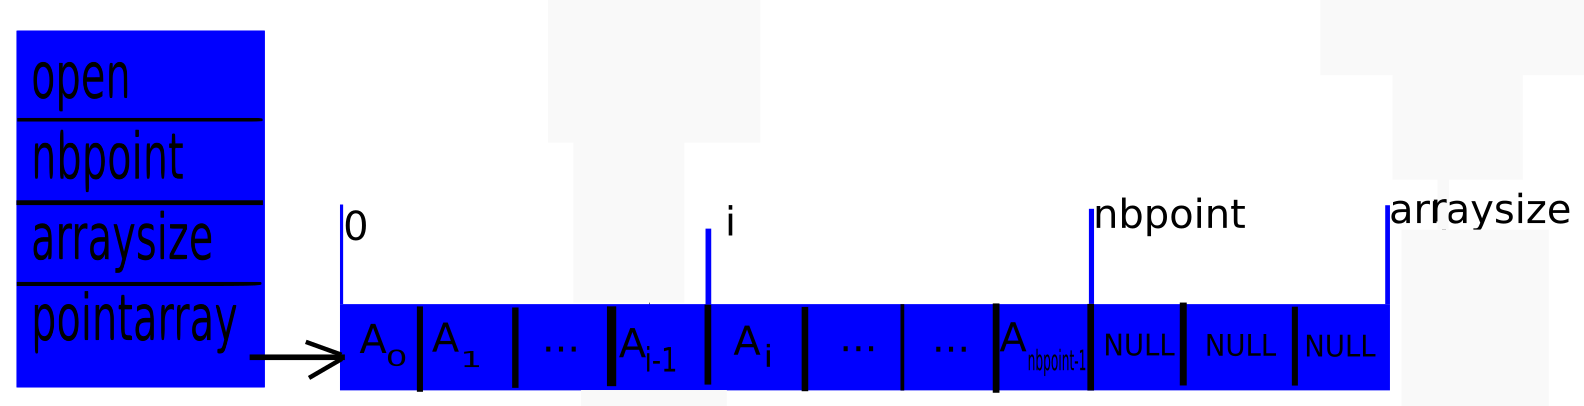
\includegraphics[height=4cm, width=14cm]{tab1.png}

\subsubsection{Fonctions et procédures}

\begin{lstlisting}[escapeinside={(*}{*)}]
/* 
 * @pre: (*\color{blue}{A != NULL $\land$ B != NULL $\land A != NULL$}*)
 * @post: (*\color{blue}{$A=A_0$ $\land$ $B=B_0$ $\land$ P->open=True $\land$ create\_Polyligne(P) = P $\land$ }*)
 * (*\color{blue}{P->nbpoint = NbrPoint(P) }*)
 */
Polyligne* CreatePolyligne(Point2D* A, Point2D* B);
/* 
 * @pre: (*\color{blue}{P != NULL}*)
 * @post: (*\color{blue}{$P=P_0$ $\land$ P->open = True $\land$  $P->nbpoint = P_0->nbpoint - 1 $*)
 */
void Open(Polyligne* P);
/* 
 * @pre: (*\color{blue}{P != NULL }*)
 * @post: (*\color{blue}{$P=P_0$ $\land$ P->open = False $\land$ $P->nbpoint = P_0->nbpoint +1 $ *)
 */
void Close(Polyligne* P);
/* 
 * @pre: (*\color{blue}{P != NULL }*)
 * @post: (*\color{blue}{$P=P_0$ $\land$ IsOpen(P)=P->open*)
 */
void IsOpen(Polyligne* P);
/* 
 * @pre: (*\color{blue}{P != NULL }*)
 * @post: (*\color{blue}{$P=P_0$ $\land$} NbrPoint(P) = P->nbpoint *)
 */
unsigned NbrPoint(Polyligne* P);
/* 
 * @pre: (*\color{blue}{P != NULL  $\land$  number < nbpoint }*)
 * @post: (*\color{blue}{$P=P_0 \land GetPoint(P) = {A_{number}} $}*)
 */
Point2D GetPoint(Polyligne* P, unsigned number);
/*
 * @pre: (*\color{blue}{ P != NULL $\land$ A != NULL }*)
 * @post: (*\color{blue}{$A=A_0$ $\land$} \color{blue}{$P->nbpoint = P_0->nbpoint + 1$  *)
 */
void AddPoint2D(Polyligne* P, Point2D* A);
/*
 * @pre: (*\color{blue}{ P != NULL $\land$ A != NULL }*)
 * @post: (*\color{blue}{$A=A_0 \land P->nbpoint = P->nbpoint - 1 $}*)
 */
void DeletePoint2D(Polyligne* P);
\end{lstlisting}

Les fonctions et procédures reprisent ci-dessus ne nécessitent pas d'invariant spécifique. On pourrait imaginer qu'il en faut un pour l'ajout et la suppression d'un point mais nous prenons la décision de n'ajouter et de supprimer que le dernier point à chaque appel de cette fonction. 

\subsubsection{Invariant et spécifications: Length}

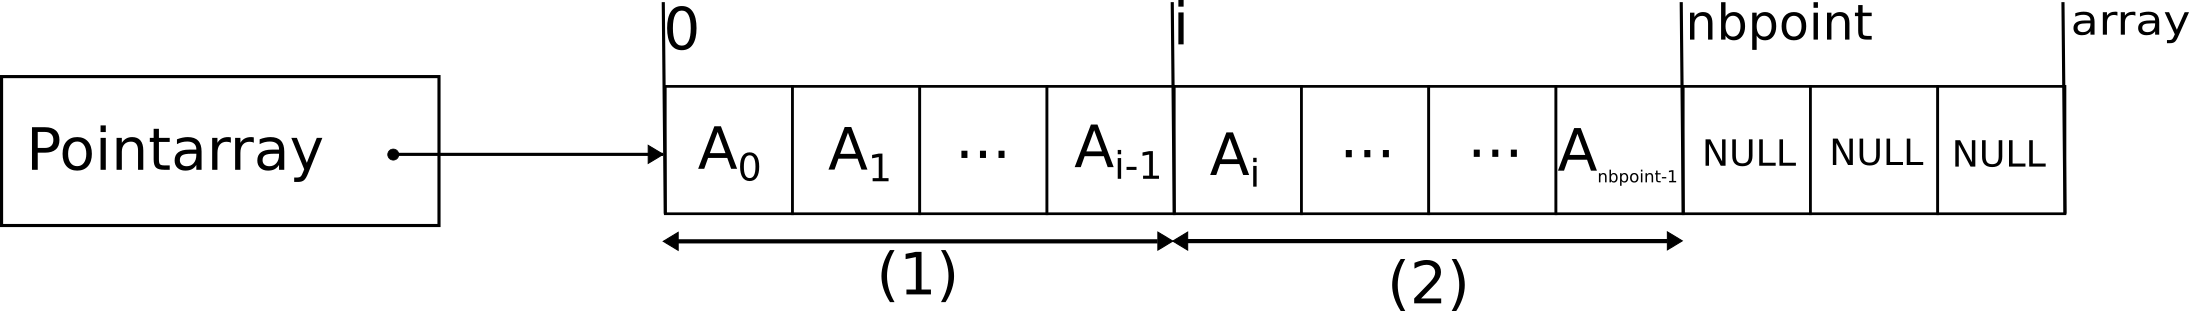
\includegraphics[scale=0.8]{inv1.png}

(1): Length = $\sum_{x=0}^{i-2} EuclDist(A_x,Ax+1)$

(2): Length à calculer

\noindent L'invariant formel qui en découle est le suivant:

\noindent$ pointArray = pointArray_0 \land \forall x, 0\leq x \leq i-2, Length =\sum_{x=0}^{i-2} EuclDist(A_x,Ax+1) \land arraySize = arraySize_0 \land nbpoint = nbpoint_0 $

\smallskip



\begin{lstlisting}[escapeinside={(*}{*)}]
/*
 * @pre: (*\color{blue}{ P != NULL}*)
 * @post: (*\color{blue}{$P=P_0$ $\land$ $Length(P)=\sum_{x=0}^{NbrPoint(P)-2} EuclDist(GetPoint(P,x),GetPoint(P,x+1)) \land P->open = P_0->open \land P->nbpoint = P_0->nbpoint$}
 *)
 */
 float Length(Polyligne* P);
\end{lstlisting}

\subsubsection{Invariant et spécifications: PolyTranslate}

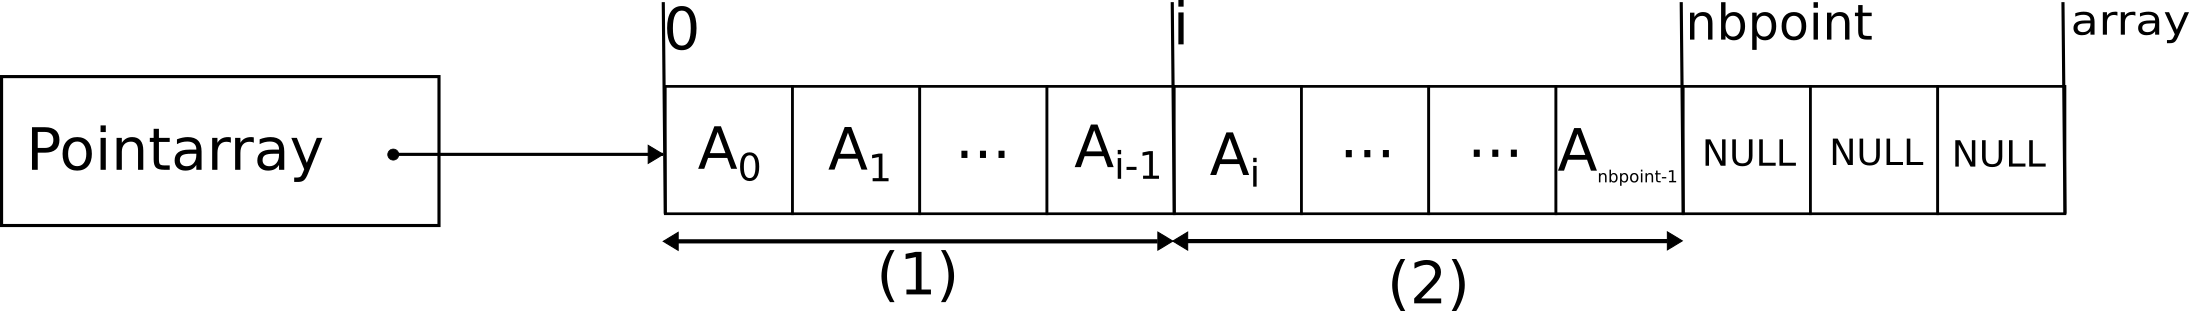
\includegraphics[scale=0.8]{inv1.png}

(1): La translation de chaque point est effectuée

(2): Translation à appliquer sur les points restants

\noindent L'invariant formel qui en découle est le suivant:

\noindent$ \forall x, 0\leq x \leq i-1, A_x = Translate((A_x)_0, K)\footnote{K est le point de référence lors de cette Translation})  \land arraySize = arraySize_0 \land nbpoint = nbpoint_0 $

\smallskip



\begin{lstlisting}[escapeinside={(*}{*)}]
/*
 * @pre: (*\color{blue}{ $P != NULL \land K != NULL$} *)
 * @post: (*\color{blue}{$P=P_0$ $\land$ $K=K_0 \land  \forall x, 0\leq x \leq P-> nbpoint-1, A_x = Translate((A_x), K)  $}
 *)
 */
 Polyligne* PolyTranslate(Polyligne* P, Point2D K);
\end{lstlisting}


\subsubsection{Invariant et spécifications: PolyRotate}

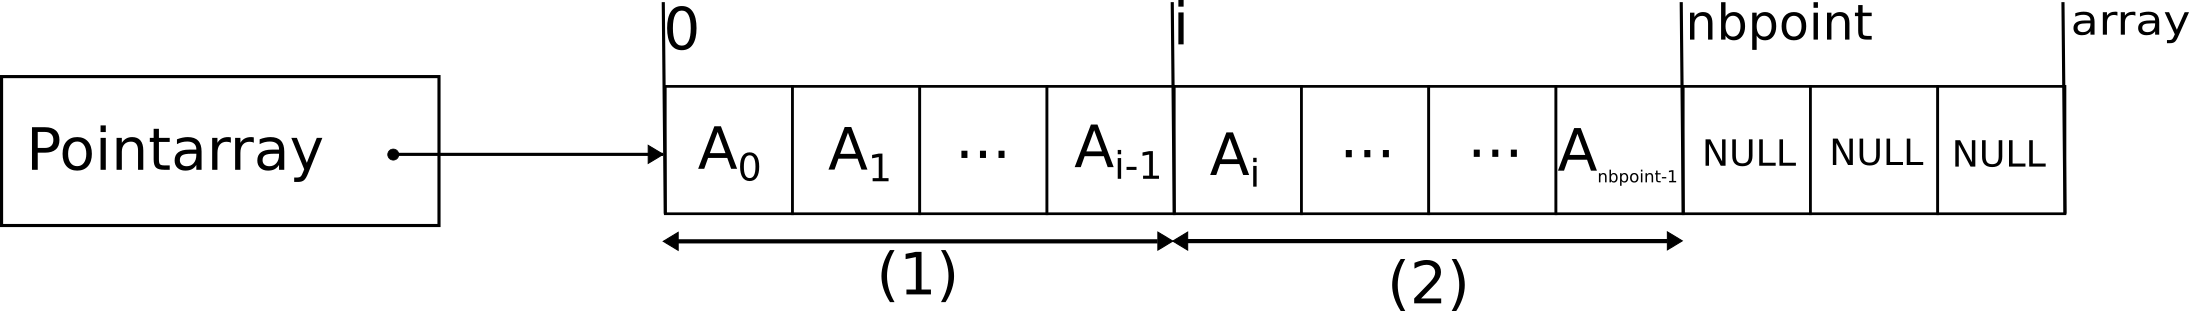
\includegraphics[scale=0.8]{inv1.png}

(1): La rotation de chaque point est effectuée

(2): Rotation à appliquer sur les points restants

\noindent L'invariant formel qui en découle est le suivant:

\noindent$ \forall x, 0\leq x \leq i-1, A_x = Rotate((A_x)_0, K, u)\footnote{K est le point de référence lors de cette Rotation et u est l'anglede référence de cette rotation})  \land arraySize = arraySize_0 \land nbpoint = nbpoint_0 $

\smallskip

\begin{lstlisting}[escapeinside={(*}{*)}]
/*
 * @pre: (*\color{blue}{ $P != NULL \land K != NULL$} *)
 * @post: (*\color{blue}{$P=P_0$ $\land$ $K=K_0 \land u = u_0\land  \forall x, 0\leq x \leq P->nbpoint-1, A_x = Rotate(A_x, K, u)  $}
 *)
 */
 Polyligne* PolyRotate(Polyligne* P, Point2D K, float u);
\end{lstlisting}

\subsection{Implémentation par liste chainée}

\subsubsection{Structure}

La structure Point2D est déjà définie plus haut mais il  est important de préciser qu'inclure cette structure(Point2D) dans une liste chaînée nécessite de définir une nouvelle structure représentant chaque cellule au sein de la liste. Notre liste est doublement chaînée ce qui implique que chaque cellule à un pointeur vers la cellule suivant mais aussi un pointeur vers la cellule précédente. 

\begin{lstlisting}
struct cell_t{
    cell* prev;
    Point2D *data;
    cell* next;

};
\end{lstlisting}


Nous décidons de donner une cellule d'en-tête à notre liste afin d'avoir accès à des données utiles comme la longueur de la polyligne, le nombre de points qui la composent et l'état d'ouverture. Dans cette cellule d'en-tête, nous mettons nos accès à notre liste: Un pointeur vers la première cellule (head) et un pointeur vers la dernière cellule (tail). 
\begin{lstlisting}
struct Polyligne_t{
    Boolean open;
    unsigned int nbpoint;
    float length;
    cell* head;
    cell* tail;
};
\end{lstlisting}

Voici un schéma représentant le structure polyligne implémentée par une liste chaînée.

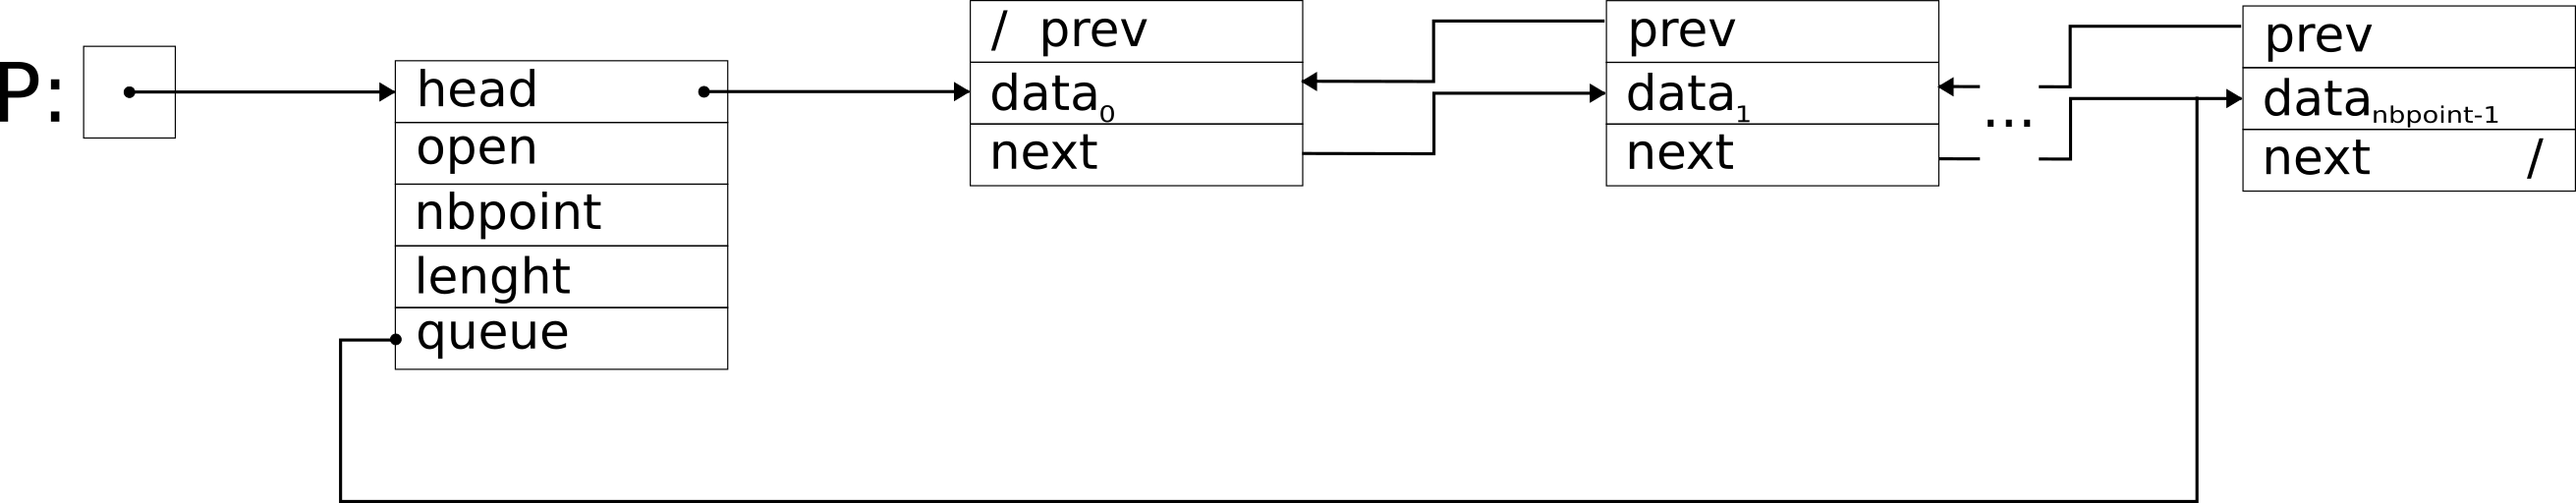
\includegraphics[scale=0.7]{schemalist.png}

\subsubsection{Fonctions et procédures}

Les spécifications des fonctions et des procédures sont semblables à l'implémentation par tableau, nous allons juste reprendre deux schémas qui expliquent le fonctionnement des fonctions qui nécessitaient un invariant. Deux schémas et non trois car la longueur de notre polyligne sera stockée dans la cellule d'en tëte de notre liste. Il ne sera donc plus nécessaire de parcourir toute la liste afin de la calculer

\paragraph{AddPoint}
\smallskip

Souvenons nous que notre fonction d'ajout va ajouter notre nouveau point à la fin de la liste. Les étapes pour cela seront les suivantes:
\begin{itemize}
    \item[1] copier le point entré en argument dans le champ utile d'une nouvelle cellule
    \item[2] Initialiser le champ "next" de la denière cellule vers la nouvelle
    \item[3] Initialiser le champ "prev" de la nouvelle cellule vers la dernière
    \item[4] Stocker l'adresse de notre nouvelle cellule dans le pointeur de fin de la cellule d'en-tête(tail).
\end{itemize}

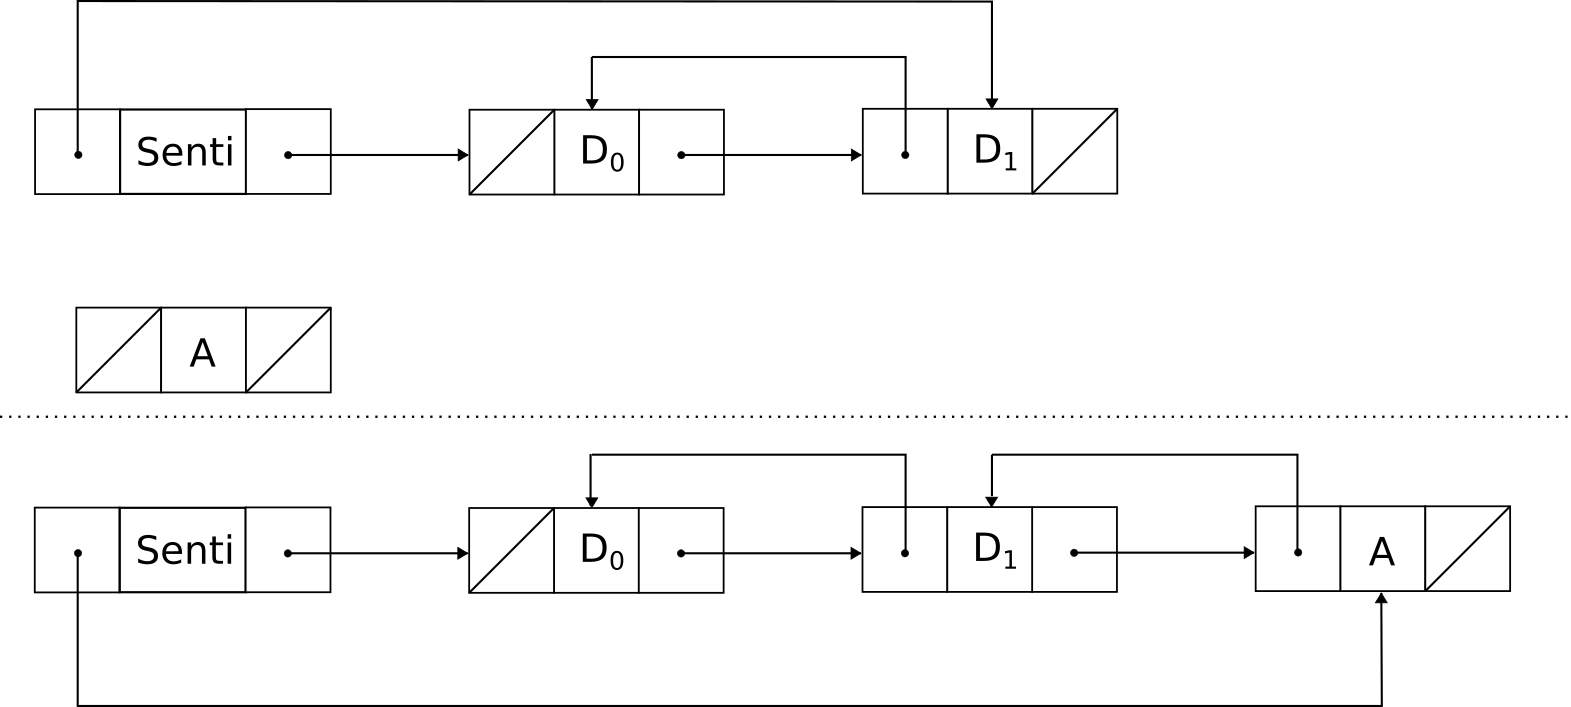
\includegraphics[scale=0.8]{Add.png}


\paragraph{SuppPoint}
\smallskip

Souvenons nous que notre fonction de suppression va supprimer le dernier point de la liste. les étapes pour cela seront les suivantes:
\begin{itemize}
    \item[1] copier la dernière de la liste dans une nouvelle cellule
    \item[2] vider le champ utile de la dernière cellule
    \item[3] vider le champ "next" de la dernière cellule
    \item[4] Stocker le champ "prev" de notre nouvelle cellule dans le pointeur de fin de la cellule d'en-tête(tail)
    \item[5] supprimer la nouvelle cellule
\end{itemize}




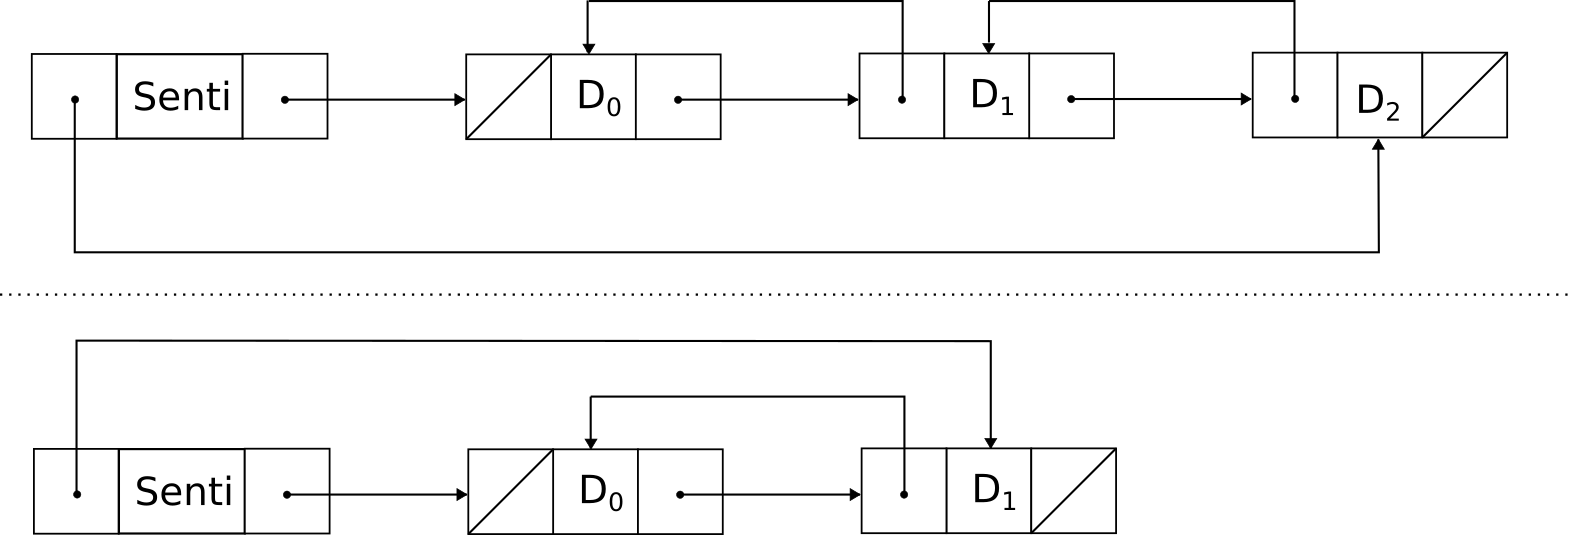
\includegraphics[scale=0.7]{supp.png}

\subsubsection{Justification des constructions récursives}



\paragraph{GetPoint}

Nous pouvons répondre à la première question de la construction récursive par l'affirmativee car la fonction GetPointRec(P, x) prend en entrée le point courant dans le parcours de la Polyligne mais aussi l'indice du point que l'on veut dans la polyligne. Cet indice semble parfait pour être notre paramètre récursif.

Ce Paramètre étant un nombre, il est aisé de trouver un cas de base à notre problème: x=0.

On peut exprimer récursivement le problème. Lorsque x est égal à 0, Il nous suffit de retourner le point courant passé en paramètre. Dans les autres cas, on rappelle la fonction avec l'indice diminué de 1.


\paragraph{PolyTranslateRec ET PolyRotateRec}
Ces deux fonction étant relativement semblable dans leur approche constructive, Nous les traiterons ensemble. Ces deux fonctions sont des fonctions pour lesquelles la récursivité nous sert à parcourir la polyligne. Le paramètre récursif est donc la cellule sur laquelle on applique la fonction. 

Le cas de base est le cas où la cellule courante est la dernière cellule, à savoir, le cas où $C->next$ == NULL.

Quand $C->next$ == NULL, nous appliquons la translation/rotation de type "point2d" sur le point courant. Dans les autre cas, nous rappelons notre fonction récursive avec la cellule suivante ($-next$) dans la polyligne. Notre problème est donc défini récursivement.


\section{Complexité}
Dans cette section nous allons uniquement nous intéresser aux processus dont la complexité change selon l'implémentation
\subsection{GetPoint}
\subsubsection{Implémentation par tableau}

\begin{lstlisting}
Point2D* GetPoint(Polyligne* P, unsigned int number){
    assert(P!=NULL && number < P->nbpoint);

    return P->pointArray[number];
}//end GetPoint()
\end{lstlisting}
Ici, la complexité est triviale. Ce processus ne comporte que deux instructions. Elle est donc \textbf{constante} $(O(2))$ 



\subsubsection{Implémentation par liste}
En comparaison, le processus GetPoint pour l'implémentation sous forme de liste se définit comme suis: 

\begin{lstlisting}
static Point2D* GetPointRec(cell* C, unsigned int number){
    if(number==0)
        return(C->data);
    else{       
        return(GetPointRec(C->next, number-1));
    }
}

Point2D* GetPoint(Polyligne* P, unsigned int number){
    assert(P!=NULL && number < P->nbpoint);

    if(P->tail==NULL)
        return NULL;

    return GetPointRec(P->head, number);
}//end GetPoint()
\end{lstlisting}
La fonction appelée en premier est GetPoint. Cette dernière est de complexité constante car elle ne réalise qu’une simple comparaison, et un appel à une autre fonction GetPointRec. C’est cette fonction qui va  nous intéresser en particulier.

\bigskip

On y trouve une structure $if$  $else$. Sous le $if$, se cache le cas de base, qui est un unique \texttt{return}, de complexité 1.
Ensuite sous le $else$, l’appel récursif.  L’appel se fait en diminuant à chaque fois l'argument \texttt{number} d’une seule unité. \texttt{number} étant le paramètre évalué pour déterminer le cas de base (number == 0) , le nombre d’appel sera toujours plus petitque  N le nombre d’élément dans notre polyligne. 
La complexité de cette partie vaut donc  $O(N)$.
Au total, nous avons une complexité \textbf{linéaire.} 



\subsection{Lenght}
\subsubsection{Implémentation par tableau}
\begin{lstlisting}
float Length(Polyligne* P){
    assert(P!=NULL);

    float length = 0;

    for(unsigned int i=0; i<P->nbpoint-1; i++){
        length += EuclDist(P->pointArray[i], P->pointArray[i+1]);
    };

    return length;
}//end Length()
\end{lstlisting}
Cette fonctions ne contient que quelques instructions simples, et une boucle appelant $nbpoint-1$ fois la fonction \texttt{EuclDist}, qui permet de calculer la distance euclidienne entre deux points, et qui n'est composé que d'instructions simples elle aussi. 
Au total nous obtenons donc :
\begin{align}
  O &= 2 + ((nbpoint-1) \times 1) + 1 \nonumber \\
       &= (nbpoint-1) + 3 \nonumber \\
\end{align}
Borné par $O(nbpoint-1)$.
\\La complexité est donc \textbf{linéaire}

\subsubsection{Implémentation par liste}
\begin{lstlisting}
float Length(Polyligne* P){
    assert(P!=NULL);
    
    return(P->length);
}//end length()
\end{lstlisting}
La longueur de la polyligne étant stocké dans la cellule d'en-tête, et actualisé à chaque modification de la taille (ajout ou suppression d'un point), il nous suffit d'accéder à ce champ. 
Il s'agit d'un instruction simple. La complexité est donc \textbf{constante}. $O(1)$

\section{Tests unitaires}



\section{Comparaison de la liste et du tableau.}

Le Problème qui nous a le plus sauté aux yeux dans l'implémentation par tableau est la taille limitée et prédéfinie du tableau. 

Etant limitée, nous devons en permanence vérifier que nous n'avons pas rempli le tableau quand on souhaite ajouter un nouveau point. Si c'est le cas, alors, nous devons faire appel à une fonction statique de ré-allocation de mémoire pour agrandir notre tableau

De l'autre coté, le fait que la taille soit prédéfinie nous amène, la majorité du temps, à avoir des cases vides dans notre tableau comme on peut le voir dans le schéma représentant notre structure dans la section 3.3.5. Nous devons aussi tenir deux tailles à jour au lieu d'une seule: le nombre de point et la taille du tableau.

L'implémentation par tableau a des inconvénients mais elle a aussi des avantages! Elle permet d'éviter la récursivité dans plusieurs fonction: la translation , la rotation, l'accesseur à un point. Dans le cas de l'accesseur, on voit même que cette implémentation permet de passer d'une complexité linéaire à une complexité constante.

\end{document}
